\subsubsection{Confusion Matrix}

A confusion matrix is a compact representation for classification results.
On the y-axis the truth values $T_*$ of a class are defined and on the x-axis the hypothesis $H_*$ produced by the underlying classifier.
When the truth class and the hypothesis match, which is the case on the diagonal of the matrix, this results in a \ac{TP}.
The other case is when the hypothesis does not match the truth value, which can be seen for each class to the left and the right side of the diagonal this is called a \ac{FP}.
The number of \ac{FN} and \ac{TN} is not presented in the confusion matrix.
\acp{FN} are the number of missing correct predictions, i.e. $FN = TP_{Should} - TP_{Is}$.
Further, \acp{TN} are the number of all possible predictions

- TODO

Further, in the context of object detection \acp{TP} and \acp{FP} are obtained by measuring the overlap of two bounding boxes, i.e. bounding box $A$ and $B$ are considered to be a \ac{TP} when $IoU(A, B) > threshold$ and the predicted classes of $A$ and $B$ matches, else it is an \ac{FP} candidate.
\ac{FP} candidate means that first all predicted bounding boxes have to be checked and mapped against a \ac{TP}, only after that the \ac{FP} candidates can be checked whether they were mapped against a \ac{TP}

- TODO that sucks


\begin{table}
\begin{center}
\begin{tabular}{c | c c c c | c}
    & \textbf{$H_1$} & \textbf{$H_2$} & \textbf{\ldots} & \textbf{$H_C$} & {$\Sigma$} \\
    \hline
    $T_1$ & \cellcolor{green}$n_{11}$ & $n_{12}$ & \ldots & $n_{1C}$ & $N_1$\\
    $T_2$ & $n_{21}$ & \cellcolor{green}$n_{22}$ & \ldots & $n_{2C}$ & $N_2$\\
    \textbf{$\vdots$} & $\vdots$ & $\vdots$ & \cellcolor{green}$\ddots$ & $\vdots$ & \textbf{$\vdots$} \\
    $T_C$ & $n_{C1}$ & $n_{C2}$ & \ldots &\cellcolor{green} $n_{CC}$ & $N_C$\\
    \hline
    $\Sigma$  & & & & & $N$\\
\end{tabular}
\caption{A Confusion Matrix}
\label{tab:confmat}
\end{center}
\end{table}

\subsubsection{Precision}

The precision metric (eq. \ref{eq:precision}) states the proportion of all correct identified samples (\ac{TP}) in relation to all positive identified samples.

\begin{equation}
    Precision = \frac{TP}{TP + FP}
    \label{eq:precision}
\end{equation}

\subsubsection{Recall}

The recall metric (eq. \ref{eq:recall}) states the proportion of all correct identified samples in relation to all possible positive samples.

\begin{equation}
    Recall = \frac{TP}{TP + FN}
    \label{eq:recall}
\end{equation}

% \subsubsection{F1-Score}

% - TODO maybe

% \subsubsection{Accuracy}

% - TODO maybe

\subsubsection{Average Precision (AP)}

\ac{AP} is mostly used in the context of object detection and is calculated for each class separately.
It is calculated by taking a set of \ac{IoU} thresholds normally ranging from $0.5$ to $0.95$ in $0.05$ steps, and calculating the recall and the precision scores with each \ac{IoU} threshold.
The resulting tuples of (recall, precision) are now sorted ascending by the recall value.
The resulting precision-recall curve could then look like the one in fig. \ref{fig:pr_curve}.
The \ac{AP} is then the area under the curve and is calculated
by taking the integral over the domain of the curve (eq. \ref{eq:ap}).

\begin{equation}
    AP = \int_0^1 Precision(Recall) dr
    \label{eq:ap}
\end{equation}

\begin{figure}
\begin{center}
    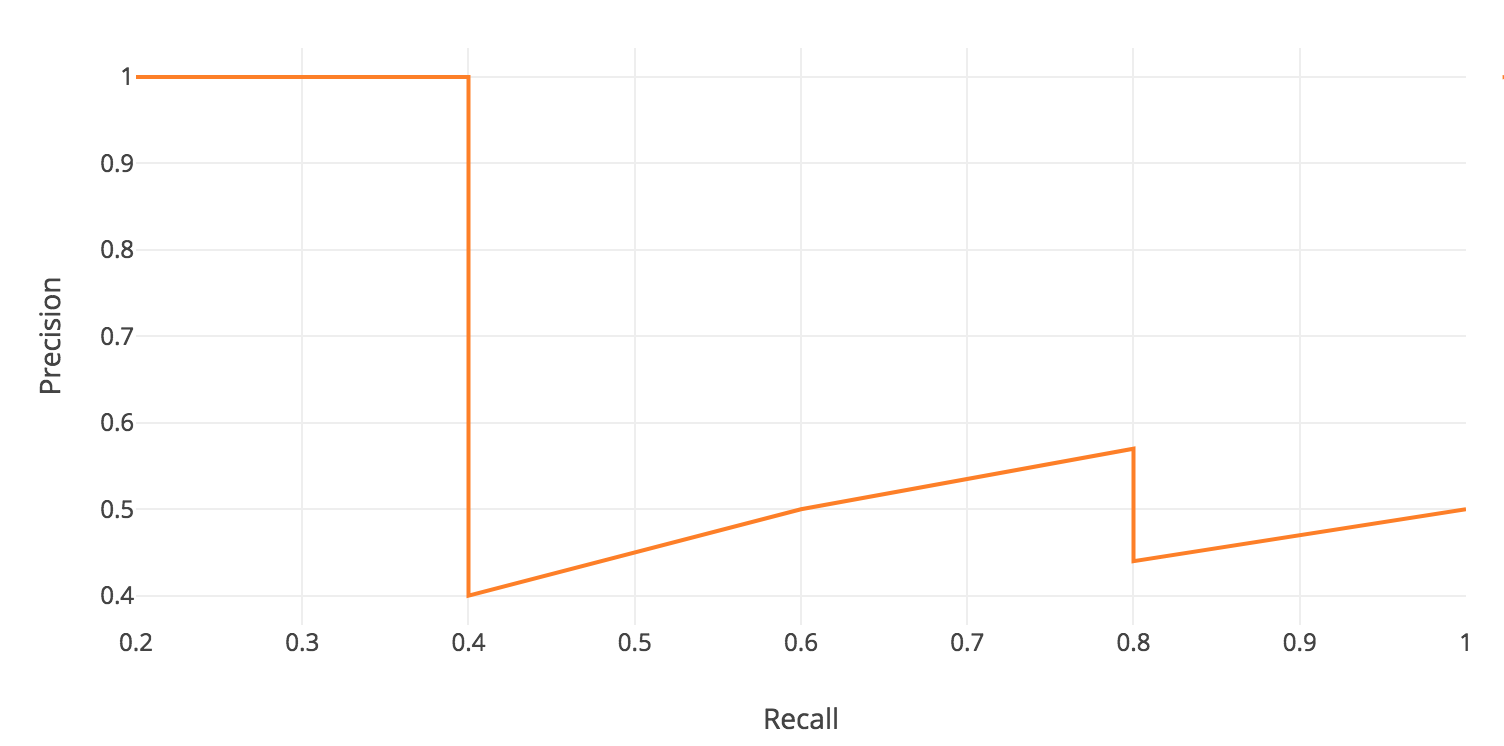
\includegraphics[width=14cm]{imgs/pr_curve.png}
    \caption{Example of a precision-recall curve, where precision and recall were calculated for different \ac{IoU} thresholds and sorted and plotted by their recall values \cite{map_article}}
    \label{fig:pr_curve}
\end{center}
\end{figure}

\subsubsection{Mean Average Precision (mAP)}

An extension of the \ac{AP} metric is the \ac{mAP}, which measures overall classification performance for all classes combined.
It is calculated as the mean of all classwise \acp{AP}, where $N$ is the number of classes (eq. \ref{eq:map}).

\begin{equation}
    mAP = \frac{1}{N} \Sigma_{i=1}^N AP_i
    \label{eq:map}
\end{equation}

\subsubsection{Mean Intersection over Union (mIoU)}

\ac{mIoU} is a metric often used in segmentation tasks.
As the name suggests it measures the \ac{IoU} between the predicted mask and the ground truth mask.
Further, the mean of all \ac{IoU} values is calculated over the number of measured samples $N$ and results in the final \ac{mIoU} value (eq. \ref{eq:miou}).

\begin{equation}
    mIoU = \frac{1}{N} \Sigma_{i=0}^{N} IoU_i
    \label{eq:miou}
\end{equation}
